\tikzstyle{mynodestyle} = [ font={}, shape=circle, minimum size=0.5cm, text=black, draw=black!55, top color=black,bottom color=black!80, text width=0.5cm, align=center]
\usetikzlibrary{shadows}
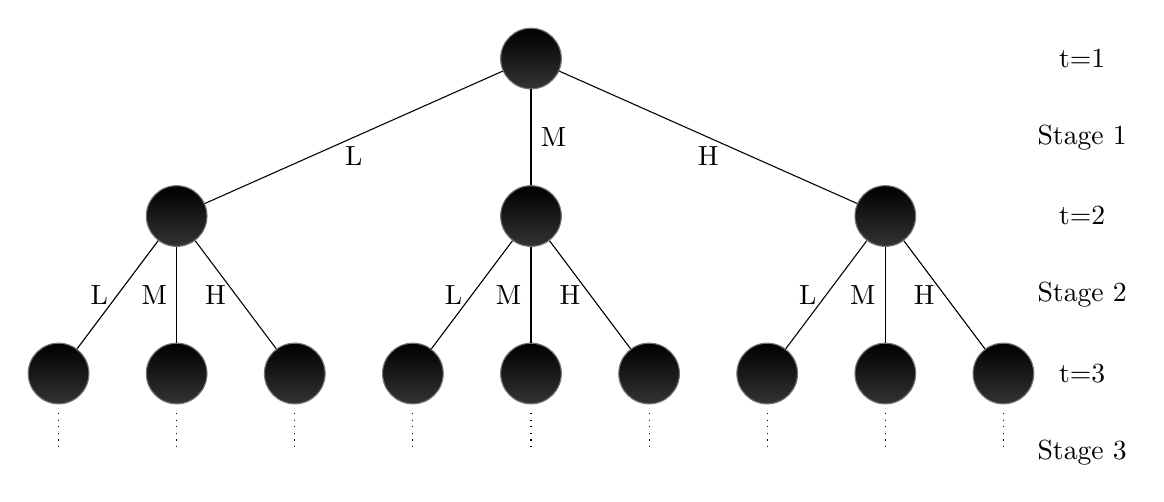
\begin{tikzpicture}

\node[mynodestyle] (v2) at (-1,5.5) {};
\node[mynodestyle] (v1) at (-5.5,3.5) {};
\node[align=left] at (6,5.5) {t=1};
\node[align=left] at (6,4.5) {Stage 1};
\node[align=left] at (6,3.5) {t=2};
\node[align=left] at (6,2.5) {Stage 2};
\node[align=left] at (6,1.5) {t=3};
\node[align=left] at (6,0.5) {Stage 3};
\node[mynodestyle] (v3) at (3.5,3.5) {};

\node[mynodestyle] (v4) at (-1,3.5) {};

\node[mynodestyle] (v5) at (-7,1.5) {};
\node[mynodestyle] (v6) at (-5.5,1.5) {};
\node[mynodestyle] (v7) at (-4,1.5) {};
\node[mynodestyle] (v9) at (-1,1.5) {};
\node[mynodestyle] (v10) at (-2.5,1.5) {};
\node[mynodestyle] (v8) at (0.5,1.5) {};
\node[mynodestyle] (v11) at (3.5,1.5) {};
\node[mynodestyle] (v12) at (2,1.5) {};
\node[mynodestyle] (v13) at (5,1.5) {};


\draw[below] (v2) edge node {L} (v1);
\draw[below] (v2) edge node[right] {M} (v4);
\draw[below] (v2) edge node {H} (v3);

\draw[below] (v6) edge node[left] {M} (v1);
\draw[below] (v5) edge node[left] {L} (v1);
\draw[below]  (v7) edge node[left] {H} (v1);
\draw[below]  (v8) edge node[left] {H} (v4);
\draw[below] (v4) edge node[left] {M} (v9) ;
\draw[below]  (v4) edge node[left] {L} (v10);
\draw[below] (v3) edge node[left] {M} (v11);
\draw[below]   (v12) edge node[left] {L} (v3);
\draw[below]  (v13) edge node[left] {H} (v3);
\draw[dotted] (-7,1) -- (-7,0.5);
\draw[dotted] (-5.5,1) -- (-5.5,0.5);
\draw[dotted] (-4,1) -- (-4,0.5);
\draw[dotted] (-2.5,1) -- (-2.5,0.5);
\draw[dotted] (-1,1) -- (-1,0.5);
\draw[dotted] (0.5,1) -- (0.5,0.5);
\draw[dotted] (2,1) -- (2,0.5);
\draw[dotted] (3.5,1) -- (3.5,0.5);
\draw[dotted] (5,1) -- (5,0.5);
\end{tikzpicture}